\documentclass{article}
\usepackage{amsmath} %This allows me to use the align functionality.
                     %If you find yourself trying to replicate
                     %something you found online, ensure you're
                     %loading the necessary packages!
\usepackage{amsfonts} 
%library(tinytex)
%tlmgr_install("hyperref")
\usepackage{hyperref}
\usepackage{lineno}
\usepackage{fancyvrb}
\linenumbers
\usepackage[margin=1.0in]{geometry}
\usepackage{float}
\usepackage{graphicx}
\usepackage{multicol}
\newcommand{\nCr}[2]{\,_{#1}C_{#2}} % nCr
\newcommand{\nPr}[2]{\,_{#1}P_{#2}} % nPr
\usepackage{natbib}        %For the bibliography
\bibliographystyle{apalike}%For the bibliography
\usepackage{Sweave}
\begin{document}
\Sconcordance{concordance:finalExam.tex:finalExam.Rnw:%
1 20 1 1 0 378 1 1 2 1 0 1 1 1 2 1 0 1 2 1 0 1 1 1 2 1 0 1 2 4 0 1 2 3 %
1 1 3 2 0 6 1 1 2 6 0 1 1 6 0 1 1 6 0 1 1 6 0 1 2 7 0 1 2 7 0 1 1 6 0 1 %
1 6 0 1 2 7 0 1 2 7 0 1 2 7 0 1 2 7 0 1 2 7 0 1 2 8 0 1 2 45 1 1 2 1 0 %
1 2 1 0 1 1 1 2 1 0 3 1 1 2 1 4 3 0 1 7 8 0 1 2 1 1 1 -17 3 0 1 14 1 0 %
1 8 3 1 1 2 1 0 4 1 1 9 10 0 1 2 1 1 1 -3 1 8 10 1 1 7 18 0 1 1 12 0 1 %
1 22 0 1 2 25 1 1 2 1 0 1 1 8 0 1 2 1 1 3 0 1 3 4 0 1 3 24 0 1 3 35 1 1 %
10 1 2 2 1 1 2 10 0 1 2 31 1 1 4 3 0 1 2 1 0 1 2 1 0 1 1 3 0 1 2 4 1 1 %
2 1 0 1 1 5 0 1 2 1 1 6 0 1 2 2 1 1 3 2 0 1 1 6 0 1 2 4 1 1 3 2 0 4 1 6 %
0 1 2 10 1 1 2 1 0 5 1 6 0 1 2 2 1 1 2 1 0 2 1 3 0 1 2 9 1 1 2 1 0 1 1 %
5 0 1 1 6 0 1 2 3 1 1 4 3 0 1 2 1 0 1 3 4 0 1 2 1 1 1 2 10 0 1 2 1 3 7 %
0 1 2 7 0 1 2 11 1 1 3 2 0 1 1 5 0 2 1 6 0 1 2 6 1 1 2 1 0 1 1 1 7 6 0 %
1 7 5 0 1 1 3 0 1 2 1 1 1 -3 1 8 11 1 1 2 1 0 1 5 7 0 1 2 1 1 1 -3 1 8 %
13 1 1 10 1 2 2 1 1 2 10 0 1 2 3 1 1 2 16 0 1 2 9 1 1 10 1 2 2 1 1 2 10 %
0 1 2 2 1 1 2 16 0 1 2 3 1 1 2 1 0 2 1 32 0 1 2 8 1 1 4 3 0 1 8 11 0 1 %
2 7 1 1 2 1 0 1 1 4 0 1 2 5 1 1 2 1 0 1 1 13 0 1 2 15 1 1 3 2 0 2 1 2 2 %
10 0 1 2 5 1 1 3 2 0 2 1 11 0 3 2 3 1 1 2 12 0 1 2 14 1}

%set the size of the graphs to fit nicely on a 8.5x11 sheet
\noindent \textbf{MA 354: Data Analysis I -- Fall 2019}\\%\\ gives you a new line
\noindent \textbf{Final Exam:}\vspace{1em}\\
\textbf{Instructions:}
\begin{itemize}
	\item You have until December 17, at 11:59p to complete this final.
	\item While you can use all of the resources available to you,
	including me, I expect you to work on this without direct help from another
	human other than me.
\end{itemize}
\small
\textbf{\texttt{R}/\LaTeX ~Sweave notes -- this should be all that you need.}
	\begin{itemize}
		\item To run \texttt{R} and print the output.
	\begin{Verbatim}
	<<>>=
		#Rcode goes here
		#Output is automatically printed in the .pdf
	@
	\end{Verbatim}
		\textbf{Remark:} All \texttt{R} chunks must have no spaces preceding the $<<>>=$ or @ syntax. 
	
		\item Provide \texttt{R} code for plot and place the plot into our document.
	\begin{Verbatim}
	<<plotName,eval=FALSE>>=
		#Rcode for plot
		#We will call this later so make sure it has a unique name
	@
	\begin{figure}[H]
		\centering
		<<fig=TRUE,echo=FALSE>>=
		library("graphics")
		<<plotName>>
		@
		\caption{Some information about our plot} \label{Fig:plot1}
	\end{figure}
	\end{Verbatim}
	You can then reference a graph in latex using \verb|\ref{Fig:plot1}|.\\
	\textbf{Remark:} All \texttt{R} chunks must have no spaces preceding the $<<>>=$ or @ syntax. 
	\item If you wanted a one line equation that is centered like this,
	\[\widehat{y_i} = \beta_0 + \beta_1 x_{1i}+ \beta_2 x_{2i} + \epsilon\]
	you can use this \LaTeX.
	\begin{Verbatim}
	\[\widehat{y_i} = \beta_0 + \beta_1 x_{1i}+ \beta_2 x_{2i} + \epsilon\]
	\end{Verbatim}
	\item If you wanted a multiple line equation that is centered like this,
	\begin{align*}
		f_X(x) &= 90 x^8(1-x)\\
		       &= 90x^8 - 90x^9\\
	\end{align*}
	you can use this \LaTeX.
	\begin{Verbatim}
	\begin{align*}
		f_X(x) &= 90 x^8(1-x)\\
			   &= 90x^8 - 90x^9\\
	\end{align*}
	\end{Verbatim}
	\end{itemize}
\newpage
\textbf{Help:}
You can ask for information about any of the following functions that we've used by
asking \texttt{R}. For example, if I wanted help with the lm() function I would 
run ?lm() in the \texttt{R} console. Note that if you're asking a question about 
a function, its library must be loaded.\\
\begin{multicols}{3} \scriptsize
\begin{itemize}
  \item Stock R functions
  \begin{itemize}
    \item which()
    \item subset()
    \item summary()
    \item names()
    \item cumsum()
    \item apply()
    \item lapply()
    \item sapply()
    \item tapply()
    \item table()
    \item prop.table()
    \item pie()
    \item barplot()
    \item hist()
    \item density()
    \item boxplot()
    \item lines()
    \item points()
    \item jitter()
    \item legend()
    \item optim()
    \item prop.test()
    \item t.test()
    \item var.test()
    \item aov()
    \item lm()
    \item anova()
    \item tukeyHSD()
    \item p.adjust()
    \item fisher.test()
    \item chisq.test()
    \item cor()
    \item cor.test()
    \item residuals()
    \item fitted()
    \item ks.test()
    \item ecdf()
    \item poly()
    \item nls()
  \end{itemize}
    \item stringr Package
  \begin{itemize}
    \item str\_split()
  \end{itemize}
    \item extraDistr Package
  \begin{itemize}
    \item dmnom()
  \end{itemize}
    \item nleqslv Package
  \begin{itemize}
    \item nleqslv()
  \end{itemize}
    \vfill\null \columnbreak
  \item ggplot2 Package Plotting
  \begin{itemize}
    \item ggplot()
    \item geom\_bar()
    \item coord\_polar()
    \item geom\_hline()
    \item geom\_text()
    \item geom\_histogram()
    \item geom\_density()
    \item geom\_freqpoly()
    \item geom\_boxplot()
    \item geom\_jitter()
    \item geom\_violin()
    \item geom\_point()
    \item geom\_smooth()
    \item geom\_hline()
    \item geom\_vline()
    \item geom\_line()
    \item facet\_grid()
    \item coord\_flip()
    \item theme\_bw()
    \item xlab()
    \item ylab()
    \item ggtitle()
  \end{itemize}
  \item Probability Distribution
  \begin{itemize}
    \item dbinom()
    \item dhyper()
    \item dnbinom()
    \item dpois()
    \item dunif()
    \item dnorm()
    \item dlnorm()
    \item dchisq()
    \item dt()
    \item df()
  \end{itemize}
  \item gridExtra Package
  \begin{itemize}
  \item grid.arrange()
  \end{itemize}
  \item qqplotr Package
  \begin{itemize}
    \item stat\_qq\_band()
    \item stat\_qq\_line()
    \item stat\_qq\_point()
  \end{itemize}
  \item boot Package
  \begin{itemize}
  \item boot()
  \item boot.ci()
  \end{itemize}
  \item BSDA Package
  \begin{itemize}
  \item SIGN.test()
  \end{itemize}
  \item simpleboot Package
  \begin{itemize}
  \item two.boot()
  \end{itemize}
  \item RVAideMemoire Package
  \begin{itemize}
  \item mood.medtest()
  \item cramer.test()
  \end{itemize}
  \item rcompanion Package
  \begin{itemize}
  \item pairwiseMedianTest()
  \item cldList()
  \item phi()
  \item cramerV()
  \end{itemize}
  \item pairwiseCI package
  \begin{itemize}
  \item pairwiseCI()
  \end{itemize}
  \item multcomp Package
  \begin{itemize}
  \item glht()
  \item cld()
  \end{itemize}
  \item FSA Package
  \begin{itemize}
  \item dunnTest()
  \end{itemize}
  \item DescTools Package
  \begin{itemize}
  \item StuartTauC()
  \end{itemize}
  \item lmtest Package
  \begin{itemize}
  \item bgtest()
  \item bptest()
  \item lrtest()
  \item waldtest()
  \end{itemize}
  \item car Package
  \begin{itemize}
  \item vif()
  \end{itemize}
  \item MASS Package
  \begin{itemize}
  \item rlm()
  \item stepAIC()
  \end{itemize}
  \item sfsmisc Package
  \begin{itemize}
  \item f.robftest()
  \end{itemize}
  \item quantreg Package
  \begin{itemize}
  \item rq()
  \end{itemize}
  \item margins Package
  \begin{itemize}
  \item margins()
  \end{itemize}
  \item ggeffects Package
  \begin{itemize}
  \item ggeffect()
  \end{itemize}
  \item emmeans Package
  \begin{itemize}
  \item emmeans()
  \item pairs()
  \item contrast()
  \end{itemize}
  \item bestglm Package
  \begin{itemize}
  \item bestglm()
  \end{itemize}
  \item glmnet Package
  \begin{itemize}
  \item glmnet()
  \end{itemize}
  \item caret Package
  \begin{itemize}
  \item createFolds()
  \end{itemize}
  \item pscl Package
  \begin{itemize}
  \item pR2()
  \end{itemize}
  \end{itemize}
  \vfill\null
  \end{multicols}
  \newpage
  \begin{multicols}{2}
  \begin{itemize}
  \item Bernoulli Distribution
  \begin{align*}
  	f_X(x|p) &= p^x(1-p)^{1-x} I(x \in \{0,1\}) \tag*{ \textbf{[PMF]}}\\
  	E(X) &=p\tag*{\textbf{[Expected Value]}}\\
  	var(X)=&p(1-p)\tag*{\textbf{[Variance]}}\\
  \end{align*}
  \item Binomial Distribution
  \begin{align*}
  	f_X(x|n,p) &={n \choose x} p^x (1-p)^{n-x} I(x \in \{0,1,\ldots n\})\tag*{\textbf{[PMF]}}\\
  	E(X) &= np \tag*{\textbf{[Expected Value]}}\\
	  var(X) & np(1-p)\tag*{\textbf{[Variance]}}\\
  \end{align*}
  \item Hypergeometric Distribution
  \begin{align*}
  	f_X(x|N,n,m,k) &=\frac{{m \choose x}{n \choose (k-x)}}{{N \choose k}}  I(x \in \mathcal{X})\tag*{\textbf{[PMF]}}\\
  	E(X) &= \frac{km}{m+n}\tag*{\textbf{[Expected Value]}}\\
	  var(X) &= \frac{km}{m+n} ~ \frac{-n}{m+n} ~ \frac{m+n-k}{m+n-1} \tag*{\textbf{[Variance]}}\\
  \end{align*}
  \item Negative Binomial Distribution
  \begin{align*}
  	f_X(x|n,p) &={{n+x-1} \choose {x}} p^n (1-p)^{x} I(x \in \{0,1,\ldots\})\tag*{\textbf{[PMF]}}\\
  	E(X) &= \frac{n(1-p)}{p}   \tag*{\textbf{[Expected Value]}}\\
	  var(X) &= \frac{n(1-p)}{p^2} \tag*{\textbf{[Variance]}}\\
  \end{align*}
  \item Poisson Distribution
  \begin{align*}
  	f_X(x|\lambda ) &= \frac{\lambda^x e^{-\lambda}}{x!}~ I(x \in \{0,1,\ldots\}) \tag*{\textbf{[PMF]}}\\
    E(X) &= \lambda\\
    var(X) &= \lambda\\
  \end{align*}
  \item Uniform Distribution
  \begin{align*}
    f_X(x|a,b) &= \frac{1}{b-a}~ I(x \in [a,b]) \tag*{\textbf{[PDF]}}\\
    E(X) &= \frac{a+b}{2} \tag*{\textbf{[Expected Value]}}\\
    var(X) &= \frac{(b-a)^2}{12} \tag*{\textbf{[Variance]}}
  \end{align*}
  \item Gaussian Distribution
  \begin{align*}
    f_X(x|\mu,\sigma) &= \frac{1}{\sigma\sqrt{2\pi}} e^{\frac{-(x-\mu)^2}{2\sigma^2}}~ I(x \in \mathbb{R}) \tag*{\textbf{[PDF]}}\\
    E(X) &= \mu\tag*{\textbf{[Expected Value]}}\\ 
    var(X) &= \sigma^2\tag*{\textbf{[Variance]}}\\ 
  \end{align*}
  \item Log-Normal Distribution
  \begin{align*}
    f_X(x|\mu, \sigma) &= \frac{1}{x \sigma \sqrt{2 \pi}} e^{\frac{(ln(x)-\mu)^2}{2 \sigma^2}}~ I(x \in (0,\infty)) \tag*{\textbf{[PDF]}}\\
	  E(X) &= e^{\mu + \sigma^2/2} \tag*{\textbf{[Expected Value]}}\\
  	var(X) &= e^{2\mu + \sigma^2}e^{\sigma^2-1} \tag*{\textbf{[Variance]}}\\
  \end{align*}
  \item Chi-squared Distribution
  \begin{align*}
    f_X(x) &= \frac{1}{\Gamma\left(\frac{v}{2}\right)2^{v/2}} x^{\frac{v}{2}-1} e^{\frac{-x}{2}} \tag*{\textbf{[PDF]}}\\
    E(X) &= v \tag*{\textbf{[Expected Value]}}\\
    var(X) &= 2v \tag*{\textbf{[Variance]}}\\
  \end{align*}
  \item Student T distribution
  \begin{align*}
      f_T(t) &= \frac{\Gamma(\frac{v+1}{2})}{\sqrt{\pi~\Gamma(v/2)}} \left(1+\frac{t^2}{2}\right)^{-(v+1)/2}\tag*{\textbf{[PDF]}}\\
      E(X) &= 0 \tag*{\textbf{[Expected Value for $v>1$]}}\\
      var(X) &= \frac{v}{v-2} \tag*{\textbf{[Variance for $v>2$]}}\\
  \end{align*}
  \item F distribution
  \begin{align*}
    f_W(w)&=\frac{\Gamma(\frac{u+v}{2})}{\Gamma(\frac{u}{2})\Gamma(\frac{v}{2})}
\left(\frac{u}{v}\right)^{u/2}\frac{w^{\frac{u}{2}-1}}{[1+(\frac{u}{v})w]^{(u+v)/2}}~I(w>0) \tag*{\textbf{[PDF]}}\\
    E(W)&=\frac{v}{v-2} \tag{\textbf{[Expected Value for $v>2$]}}\\
    var(W)&=\left(\frac{u-2}{u}\right) \left(\frac{v}{v+2}\right) \tag{\textbf{[Variance]}}\\
  \end{align*}
  \end{itemize}
  \end{multicols}
\newpage
%%%%%%%%%%%%%%%%%%%%%%%%%%%%%%%%%%%%%%%%%%%%%%%%%%%%%%%%%%%%%%%%%%%%%%%%%%%%%%%
%%%%%%%%%%%%%%%%%%%%%%%%%%%%%%%%%%%%%%%%%%%%%%%%%%%%%%%%%%%%%%%%%%%%%%%%%%%%%%%
%%%%%%%%% Part 1
%%%%%%%%%%%%%%%%%%%%%%%%%%%%%%%%%%%%%%%%%%%%%%%%%%%%%%%%%%%%%%%%%%%%%%%%%%%%%%%
%%%%%%%%%%%%%%%%%%%%%%%%%%%%%%%%%%%%%%%%%%%%%%%%%%%%%%%%%%%%%%%%%%%%%%%%%%%%%%%
\noindent \textbf{Final Exam -- Part 1} On Homework 0, we explored recent work of biomedical researchers that
investigated how MFAP4 may help doctors diagnose fibrosis/cirrhosis
stages in Hepatitis C patients. Since Homework 0, we have learned a lot. First, we 
rehash what we did on Homework 0and then we extend our analysis.
\begin{enumerate}
\item Read the following solution key for Homework 0 very closely. Write a quick
review of the work and any comments that might improve this analysis.\\
\begin{enumerate}
    \item \textbf{(Data Summary)} Hepatitis C is a disease 
    that affects the liver. The virus that causes hepatitis C 
    is spread through blood or bodily fluids of an infected person. 
    The virus is often difficult to diagnose because there are few unique 
    symptoms. Those infected, however, sometimes experience jaundice -- a 
    condition that causes yellowing of the skin or eyes, as the liver 
    is infected.

    \cite{Bracht16} consider the human microfibrillar-associated protein 4,
    or MFAP4, and its role in disease-related tissue. Stage 0--no fibrosis; 
    Stage 1--enlarged, fibrotic portal tracts; Stage 2--periportal fibrosis 
    or portal-portal septa, but intact architecture; Stage 3--fibrosis with
    architectural distortion, but no obvious cirrhosis; and Stage 4--probable
    or definite cirrhosis.

    Previously, it has been shown that MFAP4 is a biomarker candidate for hepatic
    fibrosis and cirrhosis in hepatitis C patients. The analysis of \cite{Bracht16}
    aimed to consider the ability of MFAP4 to differentiate between stages of the 
    disease -- fibrosis stages (0-2) and cirrhosis (3-4) based on the Scheuer 
    scoring system.
    
    Below, I load the data and calculate the age of patients using the ``lubridate"
    package for \texttt{R} \citep{lubridate}.
\begin{Schunk}
\begin{Sinput}
> fn<-"http://cipolli.com/students/data/biomarker.csv"
> dat <- read.csv(file=fn, header=TRUE, sep=",")
> ###Calculate the age of each subject
> library(lubridate)
> ###Create Date Variable for Date Sampled
> dos<-mdy(dat$Date.of.sampling)
> dos.year<-year(dos)
> ###Create age Variable
> age <- dos.year - dat$Year.of.Birth
> ###Add age to original dataset
> dat<-data.frame(dat,age)
\end{Sinput}
\end{Schunk}
  \begin{enumerate}
  \item Recreate Table 1 in \href{https://www.ncbi.nlm.nih.gov/pmc/articles/PMC4932744/}{the paper}. Add a row to this table labeled ``Median age IQR."  I've provided the LaTeX code for the
  table and made the first entry so you can see how it works.\\
  \textbf{Solution:}
\begin{Schunk}
\begin{Sinput}
> ###Grab data for each fibrosis stage
> dat0<-dat[which(dat$Fibrosis.Stage==0),]
> dat1<-dat[which(dat$Fibrosis.Stage==1),]
> dat2<-dat[which(dat$Fibrosis.Stage==2),]
> dat3<-dat[which(dat$Fibrosis.Stage==3),]
> dat4<-dat[which(dat$Fibrosis.Stage==4),]
> dat012<-rbind(dat0,dat1,dat2)
> dat34<-rbind(dat3,dat4)
> tapply(X=dat$age,INDEX=dat$Fibrosis.Stage,FUN=mean) 
\end{Sinput}
\begin{Soutput}
       0        1        2        3        4 
43.75258 44.82955 51.24444 57.10448 57.32836 
\end{Soutput}
\begin{Sinput}
> tapply(X=dat$age,INDEX=dat$Fibrosis.Stage,FUN=sd)
\end{Sinput}
\begin{Soutput}
       0        1        2        3        4 
12.11407 12.64298 12.03754 10.48973 11.31021 
\end{Soutput}
\begin{Sinput}
> tapply(X=dat$age,INDEX=dat$Fibrosis.Stage,FUN=median)
\end{Sinput}
\begin{Soutput}
 0  1  2  3  4 
45 46 51 57 56 
\end{Soutput}
\begin{Sinput}
> tapply(X=dat$age,INDEX=dat$Fibrosis.Stage,FUN=IQR)
\end{Sinput}
\begin{Soutput}
   0    1    2    3    4 
16.0 17.5 19.0 14.5 16.5 
\end{Soutput}
\begin{Sinput}
> tapply(X=subset(dat$Gender,dat$Gender=="female"),
+        INDEX=subset(dat$Fibrosis.Stage,dat$Gender=="female"),FUN=length)
\end{Sinput}
\begin{Soutput}
 0  1  2  3  4 
52 85 66 36 28 
\end{Soutput}
\begin{Sinput}
> tapply(X=subset(dat$Gender,dat$Gender=="male"),
+        INDEX=subset(dat$Fibrosis.Stage,dat$Gender=="male"),FUN=length)
\end{Sinput}
\begin{Soutput}
 0  1  2  3  4 
45 91 69 31 39 
\end{Soutput}
\begin{Sinput}
> tapply(X=dat$Gender,INDEX=dat$Fibrosis.Stage,FUN=length)
\end{Sinput}
\begin{Soutput}
  0   1   2   3   4 
 97 176 135  67  67 
\end{Soutput}
\begin{Sinput}
> table(dat$HCV.Genotype)
\end{Sinput}
\begin{Soutput}
            1      2      3      4 andere 
    64    389     19     60      9      1 
\end{Soutput}
\begin{Sinput}
> tapply(X=subset(dat$HCV.Genotype,dat$HCV.Genotype==1),
+        INDEX=subset(dat$Fibrosis.Stage,dat$HCV.Genotype==1),FUN=length)
\end{Sinput}
\begin{Soutput}
  0   1   2   3   4 
 70 126 100  50  43 
\end{Soutput}
\begin{Sinput}
> tapply(X=subset(dat$HCV.Genotype,dat$HCV.Genotype==2),
+        INDEX=subset(dat$Fibrosis.Stage,dat$HCV.Genotype==2),FUN=length)
\end{Sinput}
\begin{Soutput}
 0  1  2  3  4 
 2 12  1  1  3 
\end{Soutput}
\begin{Sinput}
> tapply(X=subset(dat$HCV.Genotype,dat$HCV.Genotype==3),
+        INDEX=subset(dat$Fibrosis.Stage,dat$HCV.Genotype==3),FUN=length)
\end{Sinput}
\begin{Soutput}
 0  1  2  3  4 
11 25 12  5  7 
\end{Soutput}
\begin{Sinput}
> tapply(X=subset(dat$HCV.Genotype,dat$HCV.Genotype==4),
+        INDEX=subset(dat$Fibrosis.Stage,dat$HCV.Genotype==4),FUN=length)
\end{Sinput}
\begin{Soutput}
1 2 3 
4 4 1 
\end{Soutput}
\begin{Sinput}
> tapply(X=subset(dat$HCV.Genotype,dat$HCV.Genotype==""),
+        INDEX=subset(dat$Fibrosis.Stage,dat$HCV.Genotype==""),FUN=length)
\end{Sinput}
\begin{Soutput}
 0  1  2  3  4 
14  8 18 10 14 
\end{Soutput}
\begin{Sinput}
> tapply(X=subset(dat$HCV.Genotype,dat$HCV.Genotype=="andere"),
+        INDEX=subset(dat$Fibrosis.Stage,dat$HCV.Genotype=="andere"),FUN=length)
\end{Sinput}
\begin{Soutput}
1 
1 
\end{Soutput}
\end{Schunk}
  \begin{table}[H]
  \centering
    \begin{tabular}{lccccccc}\hline
    Fibrosis Stage    & F0 & F1 & F2 & F3 & F4 & All\\\hline\hline
    \textbf{Age}                &&&&&&\\
    Mean age SD        & 43.75 (12.11)& 44.83 (12.64)&
                         52.24 (12.04)& 57.10 (10.49)&
                         57.33 (11.31)& 49.30 (13.08)\\
    Median age IQR     & 45 (16)      & 46 (17.5)    &
                         51 (19)      & 57 (14.5)    &
                         56 (16.5)    & 49 (18)\\
    \textbf{Gender}             &&&&&&\\
    Women              & 52           & 85           &
                         66           & 36           &
                         28           & 267\\
    Men                & 45           & 91           &
                         69           & 31           &
                         39           & 275\\
    Number of patients & 97           & 176          & 
                         135          & 67           &
                         67           & 542\\
    \textbf{HCV genotype}       &&&&&&\\
    1                  & 70           & 126          & 
                         100          & 50           &
                         43           & 389\\
    2                  & 2            & 12           & 
                         1            & 1            &
                         3            & 19\\
    3                  & 11           & 25           & 
                         12           & 5            &
                         7            & 60\\
    4                  & 0            & 4            & 
                         4            & 1            &
                         0            & 9\\
    Other              & 0            & 1            & 
                         0            & 0            &
                         0            & 1\\
    NA                 & 14           & 8            & 
                         18           & 10           &
                         14           & 64\\\hline
    \end{tabular}
    \caption{Patient cohorts characteristics, subdivided by fibrosis stage.}
  \end{table}
  \item Create several graphs that may be helpful for the researchers.\\
  \textbf{Solution:} Below, I recreate the graph from the original paper which is reported in a non-transformed
  scale; see Figure \ref{MFAP4stock}. We can see higher MFAP4 measurements for more advanced disease status.
\begin{Schunk}
\begin{Sinput}
> dat$Fibrosis.Stage2<-rep(NA,nrow(dat))
> dat$Fibrosis.Stage2[which(dat$Fibrosis.Stage==0 | dat$Fibrosis.Stage==1 | 
+                             dat$Fibrosis.Stage==2)]<-"0-2"
> dat$Fibrosis.Stage2[which(dat$Fibrosis.Stage==3 | dat$Fibrosis.Stage==4)]<-"3-4"
> boxplotDat<-data.frame(MFAP4.U.mL=c(dat$MFAP4.U.mL,dat$MFAP4.U.mL), 
+                        Fibrosis.Stage=c(dat$Fibrosis.Stage,dat$Fibrosis.Stage2))
> boxplotDat$Fibrosis.Stage<-as.factor(boxplotDat$Fibrosis.Stage)
> levels(boxplotDat$Fibrosis.Stage)
> levels(boxplotDat$Fibrosis.Stage)<-c("0","1","2","0-2","3-4","3","4")
> library("gplots")
> boxplot2(MFAP4.U.mL~Fibrosis.Stage,data=boxplotDat,
+         border=c("grey","grey","grey","black","black","grey","grey"),
+         col=c("white","white","white","grey","grey","white","white"),
+         xlab="Fibrosis Stage",ylab="MFAP4",shrink=0.7)
> stripchart(MFAP4.U.mL ~ Fibrosis.Stage, data = boxplotDat,
+            vertical = TRUE, method="jitter",
+            pch = 1,add=TRUE,
+            col=c("grey","grey","grey","black","black","grey","grey"),
+            subset=which(boxplotDat$Fibrosis.Stage!="0-2"&boxplotDat$Fibrosis.Stage!="3-4")
+ )
\end{Sinput}
\end{Schunk}
        \begin{figure}[H]
        \centering
\begin{Schunk}
\begin{Soutput}
[1] "0"   "0-2" "1"   "2"   "3"   "3-4" "4"  
\end{Soutput}
\end{Schunk}
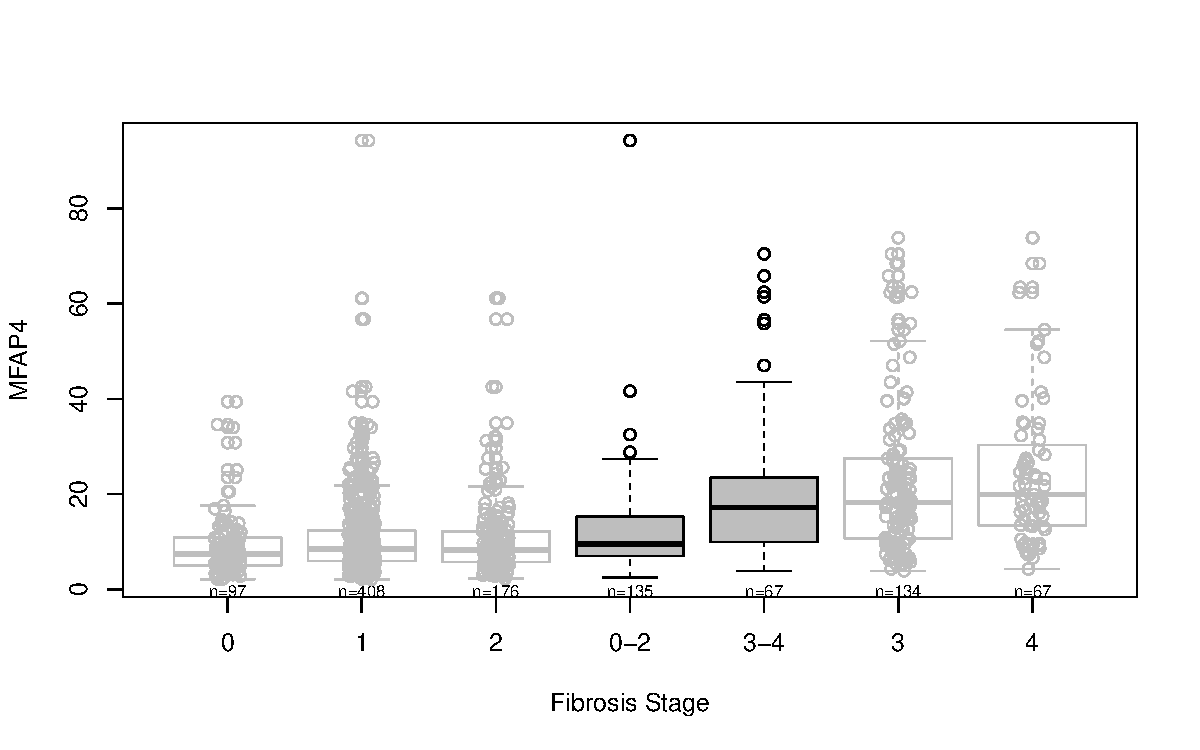
\includegraphics{finalExam-004}
        \caption{Boxplots by Fibrosis stage, grouping low and no disease (0-2) and advanced disease (3-4) as they
        did in the paper.}\label{MFAP4stock}
        \end{figure}
We can also complete plots using ggplot2 \citep{ggplot2} and gridExtra \citep{gridExtra} for R.; e.g., below we create the corresponding violin plot (Figure \ref{MFAP4gg}) that shows the distribution of MFAP4 measurements are similar for statuses 0-2 and 3-4 -- these are the groupings from the original paper.
\begin{Schunk}
\begin{Sinput}
> library(ggplot2)
> library(gridExtra)
> boxplotDat$group<-rep("notfeatured",nrow(boxplotDat))
> boxplotDat$group[which(boxplotDat$Fibrosis.Stage=="0-2")]="featured"
> boxplotDat$group[which(boxplotDat$Fibrosis.Stage=="3-4")]="featured"
> ggplot(data=boxplotDat,aes(x=Fibrosis.Stage,y=MFAP4.U.mL))+
+   geom_violin(aes(fill=group),show.legend = FALSE)+
+   geom_boxplot(width=0.25)+
+   theme_bw()+
+   xlab("Fibrosis Stage")+
+   ylab("MFAP4")+
+   ggtitle("MFAP4 by Fibrosis Stage")+
+   scale_fill_manual("", values=c("lightblue", "#DBDBDB"))
\end{Sinput}
\end{Schunk}
        \begin{figure}[H]
        \centering
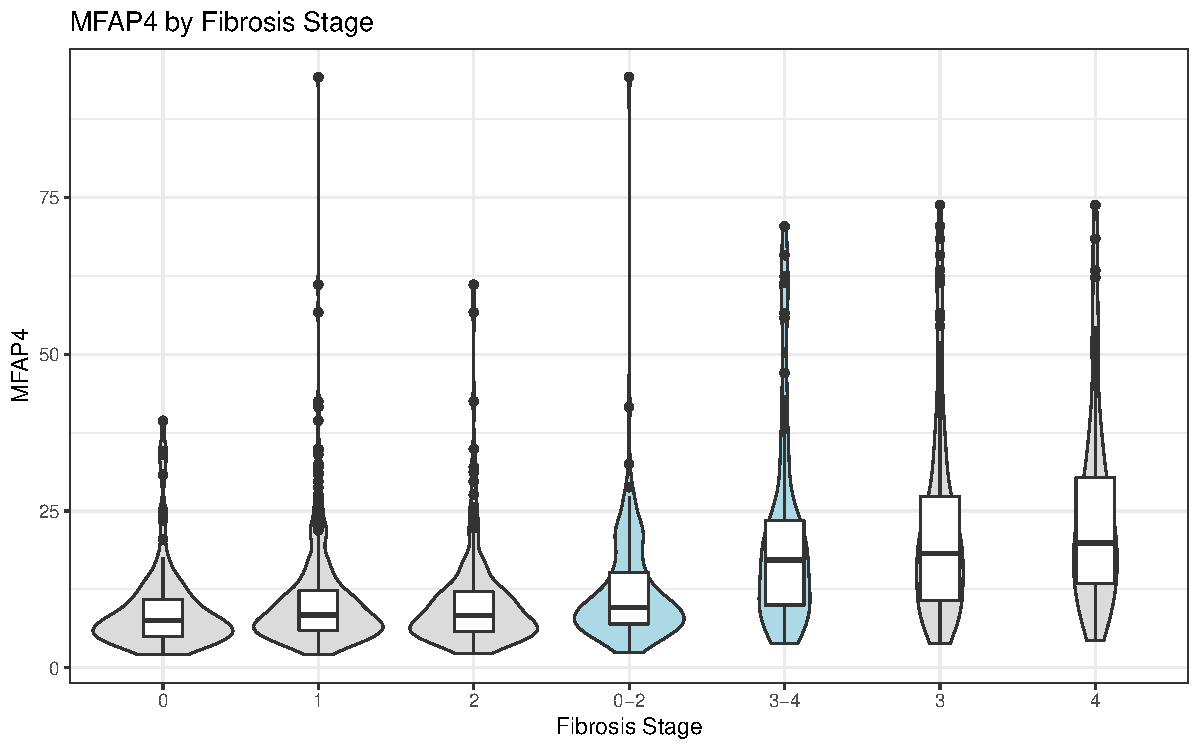
\includegraphics{finalExam-006}
        \caption{Violin plots by Fibrosis stage with box plots superimposed.}\label{MFAP4gg}
        \end{figure}
  \end{enumerate}
\end{enumerate}
\textbf{Solution:}
\newline
This code is overall very efficient and answers the question at hand. The use of \texttt{tapply()} was an efficient and concise way to gather information to construct the table and the table itself was clear. The graphs were informative, but could've been explained further. For example, the first graph on line 186 was missing a title. Also, while the question asks the researcher to explore the relationship of fibrosis and cirrhosis, it should be explained below the figures what 0-2 and 3-4 actually represent and why it is important. Not only that, but pointing out that stages 0,1,2 and how they are similar or different to 0-2 and the same for 3-4 is relevant. Being able to communicate what the data is saying and constructing a story is important for data scientists. This response could benefit from elaborating more on figures and what they mean. Especially when looking at box plots, it could be worthwhile to compare the medians and spreads of data and point out any outliers if relevant. Claims could also be elaborated on. For example, on line 184 when the researcher says "We can see higher MFAP4 measurements for more advanced disease status", they could elaborate on this by pointing to specific aspects of figures. It seems as though they see a trend and may want to investigate it further, since illustrating the data is not always enough to make a claim. Also, to make formatting more concise, they could elaborate on graphs on the same page that the graphs are on and directly below the figure, to make it easier for the reader. 
\newpage
\item Recreate Table 2 from the paper in Table \ref{MFAP4.ANOVA}. First, run an overall ANOVA as we've 
  done in class as mentioned in the caption and then use the \texttt{TukeyHSD()} 
  function to calculate the pairwise differences.
\begin{Schunk}
\begin{Sinput}
> #ggdat<-data.frame(fibrosis=dat$Fibrosis.Stage, MFAP4=dat$MFAP4.U.mL)
> #dat.f<-ggdat
> #dat.f$fibrosis<-as.factor(dat.f$fibrosis)
> #dat.f$MFAP4<-as.factor(dat.f$MFAP4)
> #anova(lm(dat$MFAP4.U.mL~dat$Fibrosis.Stage))
> anova(lm(MFAP4.U.mL~Fibrosis.Stage, data=dat))
\end{Sinput}
\begin{Soutput}
Analysis of Variance Table

Response: MFAP4.U.mL
                Df Sum Sq Mean Sq F value    Pr(>F)    
Fibrosis.Stage   1  13584 13583.9  112.67 < 2.2e-16 ***
Residuals      540  65102   120.6                      
---
Signif. codes:  0 ‘***’ 0.001 ‘**’ 0.01 ‘*’ 0.05 ‘.’ 0.1 ‘ ’ 1
\end{Soutput}
\begin{Sinput}
> anova(lm(Fibrosis.Stage~MFAP4.U.mL, data=dat))
\end{Sinput}
\begin{Soutput}
Analysis of Variance Table

Response: Fibrosis.Stage
            Df Sum Sq Mean Sq F value    Pr(>F)    
MFAP4.U.mL   1  146.1 146.102  112.67 < 2.2e-16 ***
Residuals  540  700.2   1.297                      
---
Signif. codes:  0 ‘***’ 0.001 ‘**’ 0.01 ‘*’ 0.05 ‘.’ 0.1 ‘ ’ 1
\end{Soutput}
\begin{Sinput}
> TukeyHSD(aov(lm(dat$MFAP4.U.mL~as.factor(dat$Fibrosis.Stage)), conf.level = 0.95))
\end{Sinput}
\begin{Soutput}
  Tukey multiple comparisons of means
    95% family-wise confidence level

Fit: aov(formula = lm(dat$MFAP4.U.mL ~ as.factor(dat$Fibrosis.Stage)), conf.level = 0.95)

$`as.factor(dat$Fibrosis.Stage)`
         diff        lwr       upr     p adj
1-0  1.301353 -2.4541799  5.056886 0.8777020
2-0  3.153807 -0.7991649  7.106778 0.1874077
3-0 11.741745  7.0240362 16.459454 0.0000000
4-0 15.388014 10.6703049 20.105722 0.0000000
2-1  1.852454 -1.5452808  5.250188 0.5679669
3-1 10.440392  6.1771314 14.703652 0.0000000
4-1 14.086660  9.8234000 18.349921 0.0000000
3-2  8.587938  4.1497688 13.026107 0.0000017
4-2 12.234207  7.7960375 16.672376 0.0000000
4-3  3.646269 -1.4848264  8.777364 0.2948449
\end{Soutput}
\end{Schunk}
I will run full length tests of the ANOVA in question 4 including the hypthoses and assumptions. 
    \begin{table}[H]
  \centering
    \begin{tabular}{lccccc}\hline
    Comparison & Difference & Lower Bound & Upper Bound & $p$ value\\\hline\hline
    F1-F0   & 1.301353 & -2.4541799  & 5.056886   &0.8777020\\
    F2-F0   & 3.153807 & -0.7991649  & 7.106778   &0.1874077\\
    F3-F0   & 11.741745 & 7.0240362  & 16.459454  &0.0000000\\
    F4-F0   & 15.388014 & 10.6703049 & 20.105722  &0.0000000\\
    F2-F1   & 1.852454  &-1.5452808  & 5.250188   &0.5679669\\
    F3-F1   & 10.440392 & 6.1771314  & 14.703652  &0.0000000\\
    F4-F1   & 14.086660 & 9.8234000  & 18.349921  &0.0000000\\
    F3-F2   &  8.587938 & 4.1497688  & 13.026107  &0.0000017\\
    F4-F2   & 12.234207 & 7.7960375  & 16.672376  &0.0000000\\
    F4-F3   & 3.646269 & -1.4848264  &8.777364    &0.2948449\\\hline
    \end{tabular}
    \caption{Results of the pairwise comparisons of individual
    hepatic fibrosis stages with  respect to MFAP4 values
    after significant ANOVA result.} \label{MFAP4.ANOVA}
  \end{table}
  \item Create this table again, but this time for analysis on
  the median, in Figure \ref{MFAP4.MOOD}. First, run an overall \texttt{mood.medtest()} 
  as we've done in class using package \citep{RVAideMemoire} then use the 
  \texttt{pairwiseMedianTest()} function from the ``rcompanion" 
  package \citep{rcompanion} and \texttt{pairwiseCI()} from the
  ``pairwiseCI" package \citep{pairwiseCI} to calculate the pairwise differences.
\begin{Schunk}
\begin{Sinput}
> library(RVAideMemoire)
> mood.medtest(MFAP4.U.mL~Fibrosis.Stage,data=dat)
\end{Sinput}
\begin{Soutput}
	Mood's median test

data:  MFAP4.U.mL by Fibrosis.Stage
X-squared = 71.737, df = 4, p-value = 9.755e-15
\end{Soutput}
\begin{Sinput}
> library(rcompanion)
> library(pairwiseCI)
\end{Sinput}
\end{Schunk}
\begin{Schunk}
\begin{Sinput}
> pwmt<-pairwiseMedianTest(MFAP4.U.mL~as.factor(Fibrosis.Stage), data= dat, method = "BH")
\end{Sinput}
\end{Schunk}
\begin{Schunk}
\begin{Sinput}
> pairwiseCI(MFAP4.U.mL~Fibrosis.Stage, data=dat)
\end{Sinput}
\begin{Soutput}
95 %-confidence intervals 
 Method:  Difference of means assuming Normal distribution, allowing unequal variances 
  
  
    estimate   lower  upper
1-0    1.301 -0.5501  3.153
2-0    3.154  0.9780  5.330
3-0   11.742  7.6023 15.881
4-0   15.388 11.2967 19.479
2-1    1.853 -0.2270  3.932
3-1   10.440  6.3485 14.532
4-1   14.087 10.0435 18.130
3-2    8.588  4.3449 12.831
4-2   12.234  8.0380 16.430
4-3    3.646 -1.7986  9.091
\end{Soutput}
\begin{Sinput}
> 
\end{Sinput}
\end{Schunk}
I will include the assumptions and hypotheses for the Mood's Median test in question 4.
  \begin{table}[H]
  \centering
    \begin{tabular}{lccccc}\hline
    Comparison & Difference & Lower Bound & Upper Bound & $p$ value\\\hline\hline
    F1-F0   & 3.7031 & -0.5501  &3.153   & 2.157e-01\\
    F2-F0   & 4.352 & 0.9780  & 5.330 & 4.631e-03\\
    F3-F0   &8.2787  & 7.6023  & 15.881  & < .00001\\
    F4-F0   & 8.1823 & 11.2967  & 19.479  & < .00001\\
    F2-F1   & 4.159 & -0.2270  &  3.932  & 5.805e-02\\
    F3-F1   &  8.1835 & 6.3485  & 14.532  & < .00001\\
    F4-F1   & 8.0865 & 10.0435  & 18.130  & < .00001\\
    F3-F2   & 8.4861 & 4.3449  & 12.831  &3.230e-04\\
    F4-F2   & 8.392 & 8.0380  & 16.430  & < .00001\\
    F4-F3   & 10.8896 & -1.7986  & 9.091  &1.348e-01\\\hline
    \end{tabular}
    \caption{Results of the pairwise comparisons of individual
    hepatic fibrosis stages with  respect to MFAP4 values
    after significant Mood's Median result.} \label{MFAP4.MOOD}
  \end{table}
  \item Reflect on the differences (if any) between these analyses. Also discuss
  which approach or approaches are relevant to this data and which approach
  or approaches are most appropriate. You should consider the ANOVA and Mood's 
  median analysis above, and additionally that the ANOVA was performed
  on the $\log_2($MFAP4$)$ scale. 
  \newline
  \newline
  Now we can perform the full tests of the ANOVA and the Mood's Median to compare the approaches. 
  \textbf{Hypotheses:}
  The null hypothesis for the ANOVA is that the population means of all fibrosis stages are equal. The alternative hypothesis for the ANOVA is that not all of the population means of the fibrosis stages are equal. 
  \newline \textbf{Assumptions:}
  The ANOVA has three assumptions for performing an analysis on variance: independent random samples, normality, and equal population variances.
  \begin{enumerate}
  \item \textbf{Independent Random Samples:} According to the methods of data collection from the research paper, samples were collected at different sites using a standardized protocol to reduce bias. This leads us to believe that the samples were independent and random. 
  \item \textbf{Normality:}
  \begin{figure}[H]
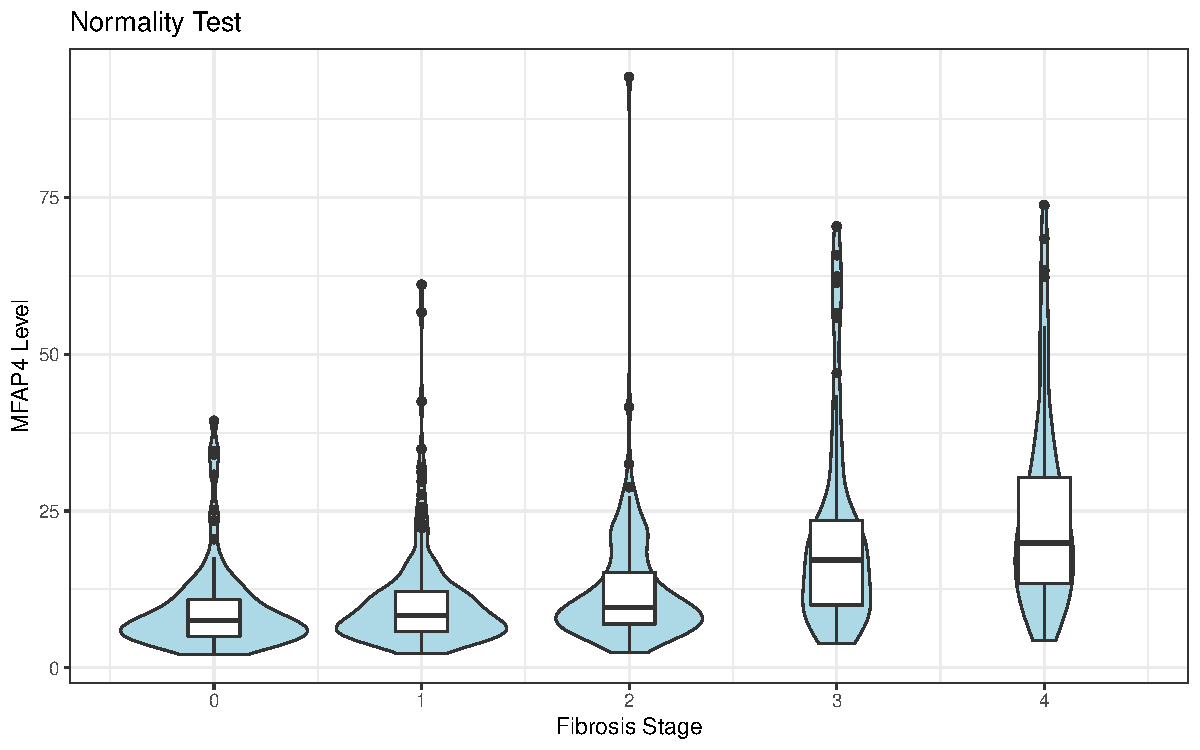
\includegraphics{finalExam-011}
\end{figure}
The graph above shows that although the data is slightly skewed for most of the stages due to outliers, none of these samples depart severely from normality to the point where we would not be able to run an ANOVA on these differing treatments. 
\item \textbf{Equal Population Variances:}
\begin{Schunk}
\begin{Sinput}
> bartlett.test(dat$MFAP4.U.mL, as.factor(dat$Fibrosis.Stage))
\end{Sinput}
\begin{Soutput}
	Bartlett test of homogeneity of variances

data:  dat$MFAP4.U.mL and as.factor(dat$Fibrosis.Stage)
Bartlett's K-squared = 103.84, df = 4, p-value < 2.2e-16
\end{Soutput}
\end{Schunk}
The results of this test are significant because the p-value is essentially zero. Since this is the case, we reject our null hypothesis that the population variances are equal and have evidence to believe that the population variances are not all equal. Therefore, this may point us to use the Mood's Median Test as a better predictor or a non parametric alternative to the ANOVA. 
\end{enumerate}
We can therefore begin our analysis evaluating the Mood's Median assumptions. The assumptions for this test are that observations are independent and representative. As was discussed before when looking at the assumptions for ANOVA, these observations are independent and representative, making the Mood's Median test a better alternative to the ANOVA for this sample. Specifically, the sample is representative because the data is collected in a way that is unbiased, implying representativeness. 

In all test cases, results were highly statistically significant. This leads me to believe that while Mood's Median is the safest test to run because it is the non parametric alternative. This exercise implies though that as long as the sample we're observing does not deviate severely from its assumptions, the ANOVA and the ANOVA log base 2 will still give us fairly similar results to the Mood's Median Test. The ANOVA tests themselves do not differ too much from each other. Since the ANOVA deviates from the equal population assumptions anyways, it does not matter if the ANOVA or the ANOVA log base 2 is chosen. Especially if the data doesn't meet the assumptions, transforming the data will not necessarily yield the results that we want. Therefore, we can conclude that Mood's Median test is the most appropriate test for this data because all of its assumptions are met. 

  \item Is MFAP4 helpful in distinguishing stage of fibrosis in hepatitis C patients?
\newline
\newline
The MFAP4 is helpful in distinguishing stage of fibrosis in hepatitis C patients as was illustrated by the tests ran above. The ANOVA log base 2, the ANOVA, and the Mood's Median test all yield statistically significant results. If we take for the ANOVA tests that our null hypothesis was that the population variances were equal, and the alternative hypothesis was that not all population variances were equal, our results yielded that we could reject the null and have evidence to believe that not all of our population variances were equal, meaning that MFAP4 is helpful in distinguishing stage of fibrosis in hepatitis C patients. The Mood's Median test yielded the same result. If our null hypothesis was that the population medians were all equal, and the alternative hypothesis was that our population medians were not all equal, we can reject the null and have evidence to believe that not all of our population medians are equal. This means that MFAP4 is helpful in distinguishing stage of fibrosis in hepatitis C patients. If we look at inter-group differences found by these tests, all tests conclude that fibrosis stages 3 and 4 are not statistically different from each other, but are statistically different from fibrosis stages 0, 1, and 2. The fibrosis stages of 0, 1, and 2 are also not statistically different from each other. Therefore, this illustrates that in particular, MFAP4 is helpful in distinguishing between fibrosis and cirrhosis in hepatitis C patients. 
\end{enumerate}
\newpage
%%%%%%%%%%%%%%%%%%%%%%%%%%%%%%%%%%%%%%%%%%%%%%%%%%%%%%%%%%%%%%%%%%%%%%%%%%%%%%%
%%%%%%%%%%%%%%%%%%%%%%%%%%%%%%%%%%%%%%%%%%%%%%%%%%%%%%%%%%%%%%%%%%%%%%%%%%%%%%%
%%%%%%%%% Part 2
%%%%%%%%%%%%%%%%%%%%%%%%%%%%%%%%%%%%%%%%%%%%%%%%%%%%%%%%%%%%%%%%%%%%%%%%%%%%%%%
%%%%%%%%%%%%%%%%%%%%%%%%%%%%%%%%%%%%%%%%%%%%%%%%%%%%%%%%%%%%%%%%%%%%%%%%%%%%%%%
\noindent \textbf{Final Exam -- Part 2}
On Homework 1, we explored recent work of psychology researchers that
investigated how subjective socioeconomic status affects how participants experience
negative and positive emotions and whether or not the effect is different by race. Since 
Homework 1, we have learned a lot. First, we rehash what we did on Homework 1
and then we extend our analysis.

\begin{enumerate}
\item Read the following solution key for Homework 1 very closely. Write a quick
review of the work and any comments that might improve this analysis.\\
\textbf{Solution:}

\begin{enumerate}
\item Load Data. There are over 100 columns, so we don't print previews of the data
like we did previously.
\begin{Schunk}
\begin{Sinput}
> ###Download data
> dat.white<-read.csv("https://cipolli.com/students/data/WhiteParticipants.txt",
+ header=T,sep=",",stringsAsFactors = FALSE)
> dat.black<-read.csv("https://cipolli.com/students/data/BlackParticipants.txt",
+ header=T,sep=",",stringsAsFactors = FALSE)
> dat.matched<-read.csv("https://cipolli.com/students/data/matchedsample.txt",
+ header=T,sep=",",stringsAsFactors = FALSE)
> colnames(dat.matched)<-c("aid","id","MatchedSample")
\end{Sinput}
\end{Schunk}
\item Remove non-White observations from \texttt{dat.white}; i.e., remove observations 
from \texttt{dat.white} where Race does not equal 1. \textbf{Also remove non-Black observations
from \texttt{dat.black}; i.e., remove observations 
from \texttt{dat.black} where Race does not equal 3.}\\
\textbf{Solution:}
\begin{Schunk}
\begin{Sinput}
> dat.white<-dat.white[dat.white$Race==1,] 
> nrow(dat.white) #1009
\end{Sinput}
\begin{Soutput}
[1] 1009
\end{Soutput}
\begin{Sinput}
> dat.black<-dat.black[dat.black$Race==3,]
> nrow(dat.black) #1838
\end{Sinput}
\begin{Soutput}
[1] 1838
\end{Soutput}
\end{Schunk}
\item Create an object called \texttt{dat.wb} that contains all of the observations;
i.e., merge the data loaded from WhiteParticipants.csv and BlackParticipants.csv.\\
\textbf{Solution:}
\begin{Schunk}
\begin{Sinput}
> #Combine Data
> dat.wb<-rbind(dat.black,dat.white)
> nrow(dat.wb) #2847
\end{Sinput}
\begin{Soutput}
[1] 2847
\end{Soutput}
\end{Schunk}
\item The aid of observations that make up a representative sample have a value of
1; i.e., observation $i$ is in the representative sample if dat.matched\$MatchedSample[$i$]
is 1. Remove observations that are not part of the representative sample from
\texttt{dat.wb}.\\
\textbf{Solution:}
\begin{Schunk}
\begin{Sinput}
> ### Keep those selected for the sample
> dat.matched<-dat.matched[which(dat.matched$MatchedSample==1),]
> matches<-match(dat.matched$aid,dat.wb$aid) #NA if no match
> matches<-matches[-which(is.na(matches))] #Remove non matches
> dat.wb<-dat.wb[matches,] #Keep those selected
> nrow(dat.wb) #1015
\end{Sinput}
\begin{Soutput}
[1] 1015
\end{Soutput}
\end{Schunk}
\item Amazon flagged 5 users as a false match for the demographic the researchers
were measuring. Remove these users from \texttt{dat.wb}; the aid of each user is 
listed below.
\begin{itemize}
\item 5c9963bd-8f12-6d35-bafc-cdeee22209ed
\item 5c996fcc-1f89-13c3-50e7-3f7c554aad3c
\item 5c9a3bd8-1cbc-854b-a193-620f5eaee500
\item 5cbcaf2e-3233-62d3-7aa3-ad1c9f4ab5a0
\item 5c9a68ff-1fd6-4ff1-6bf5-b8a1504075b8
\end{itemize}
\textbf{Solution:}
\begin{Schunk}
\begin{Sinput}
> dat.wb<-dat.wb[-which(dat.wb$aid=="5c9963bd-8f12-6d35-bafc-cdeee22209ed"),]
> dat.wb<-dat.wb[-which(dat.wb$aid=="5c996fcc-1f89-13c3-50e7-3f7c554aad3c"),]
> dat.wb<-dat.wb[-which(dat.wb$aid=="5c9a3bd8-1cbc-854b-a193-620f5eaee500"),]
> dat.wb<-dat.wb[-which(dat.wb$aid=="5cbcaf2e-3233-62d3-7aa3-ad1c9f4ab5a0"),]
> dat.wb<-dat.wb[-which(dat.wb$aid=="5c9a68ff-1fd6-4ff1-6bf5-b8a1504075b8"),]
> nrow(dat.wb) #1010
\end{Sinput}
\begin{Soutput}
[1] 1010
\end{Soutput}
\end{Schunk}
\item Create a variable called \texttt{LadderDiff} by subracting the column labeled
``LadderSelf" from the column labeled ``LadderGroup."\\
\textbf{Solution:}
\begin{Schunk}
\begin{Sinput}
> dat.wb$LadderGroup<-as.numeric(dat.wb$LadderGroup)
> dat.wb$LadderSelf<-as.numeric(dat.wb$LadderSelf)
> dat.wb$LadderDif<-dat.wb$LadderGroup-dat.wb$LadderSelf
\end{Sinput}
\end{Schunk}
\textbf{Remark:} I added \texttt{stringsAsFactors = FALSE} to the data
reading calls, so Race isn't a factor in my data frame. To me,
I find it simpler to do this than to worry about what's a factor.
If you didn't add \texttt{stringsAsFactors = FALSE} then your
LadderDif calculation isn't correct unless you coherced the data 
correctly to a numeric data type. If you didn't coherce to a
character first, you would end up subtracting the integer values
the factors are stored at; e.g., $\{1,2,3,...,10\}$ is mapped
onto $\{1,3,4,...,2\}$ which can cause some serious issues.
For example, see the below toy example.
\begin{Schunk}
\begin{Sinput}
> xx<-factor(c("1","2","3","4","5","6","7","8","9","10"))
> as.numeric(xx) #returns integer the character label is stored at
\end{Sinput}
\begin{Soutput}
 [1]  1  3  4  5  6  7  8  9 10  2
\end{Soutput}
\begin{Sinput}
> as.numeric(as.character(xx)) #returns the numeric value of the character
\end{Sinput}
\begin{Soutput}
 [1]  1  2  3  4  5  6  7  8  9 10
\end{Soutput}
\end{Schunk}
\item Create a variable called \texttt{PosEmo} by averaging the responses in columns
labeled: ``Amused", ``Awe", ``Grateful", ``Hopeful", ``Inspired", ``Interested",
``Joy", ``Love", ``Proud", ``Serene."\\
\textbf{Solution:}
\begin{Schunk}
\begin{Sinput}
> #Create a subset of the data of interest
> PosEmoSubset<- dat.wb[,c("Amused","Awe","Grateful","Hopeful","Inspired","Interested",
+                       "Joy","Love","Proud","Serene")]
> #Ensure the data is being treated as numeric
> PosEmoSubset<-apply(X=PosEmoSubset,MARGIN = 2,FUN = as.numeric)
> ## Create Variable as mean of positive emotion responses  -- ignore NA
> dat.wb$PosEmo=apply(X=PosEmoSubset,MARGIN=1,FUN=mean,na.rm=TRUE)
\end{Sinput}
\end{Schunk}
\textbf{Remark:} There is one person in the data missing all observations
in the subset of positive emotions.
\begin{Schunk}
\begin{Sinput}
> PosEmoSubset[which(is.na(dat.wb$PosEmo)),]
\end{Sinput}
\begin{Soutput}
    Amused        Awe   Grateful    Hopeful   Inspired Interested        Joy 
        NA         NA         NA         NA         NA         NA         NA 
      Love      Proud     Serene 
        NA         NA         NA 
\end{Soutput}
\end{Schunk}
There are also participants who didn't answer \emph{all} of the questions.
\begin{Schunk}
\begin{Sinput}
> #participants in row 1 and 528 didn't answer the Amused question
> which(is.na(PosEmoSubset[,1]))
\end{Sinput}
\begin{Soutput}
[1]   1 528
\end{Soutput}
\begin{Sinput}
> #participants 1, 220, 296, 528, 948 did not answer all of the questions
> which(!complete.cases(PosEmoSubset))
\end{Sinput}
\begin{Soutput}
[1]   1 220 296 528 948
\end{Soutput}
\end{Schunk}
This yields the question of whether or not these participants average
score measure the same thing as for those participants that answered
all of the questions. Certainly the participant in row 1 should be removed,
we have no information for them -- but what about the others? We kept them
because we can see the answers to these questions are highly related, but
it was after a long conversation with the researcher who finally talked 
me out of my statistical purity. The deal was made after ensuring that
the analyses yielded the same results regardless of this choice of
who to keep or remove.
\item Plot \texttt{LadderDiff} versus \texttt{PosEmo} for White participants
and for Black participants. Comment on differences in the plot.\\
\textbf{Solution:} First, we make the race variable a factor.
\begin{Schunk}
\begin{Sinput}
> #Clean data for better graphs
> dat.wb$Race<-factor(dat.wb$Race)
> levels(dat.wb$Race)
\end{Sinput}
\begin{Soutput}
[1] "1" "3"
\end{Soutput}
\begin{Sinput}
> levels(dat.wb$Race)<-c("White","Black") #1=White, 3=Black
> levels(dat.wb$Race)
\end{Sinput}
\begin{Soutput}
[1] "White" "Black"
\end{Soutput}
\end{Schunk}
In Figure \ref{Fig:marginal1}, we see there are some
differences across race. In particular we see that White
participants seem to rate themselves lower than the group
(LadderDif$>$0) at higher rates compared to Black participants
who seem to rate themselves higher than the group (LadderDif$<$0)
at higher rates compared to White participants.

\begin{Schunk}
\begin{Sinput}
> library(ggplot2)
> library(gridExtra)
> g1<-ggplot(data=dat.wb,aes(x=LadderDif,fill=Race))+
+ geom_bar(aes(y=..count../sum(..count..)),
+          position = position_dodge(preserve = "single"))+
+ geom_hline(yintercept = 0)+
+ theme_bw()+
+ xlab("Ladder Difference (Group-Self)")+
+ ylab("Density")
> g2<-ggplot(data=dat.wb,aes(x=Race,y=PosEmo))+
+ geom_violin(fill="lightblue")+
+ geom_boxplot(fill="white",width=0.25)+
+ theme_bw()+
+ xlab("Race")+
+ ylab("Positive Emotion Measure")
> grid.arrange(g1,g2,ncol=2)
\end{Sinput}
\end{Schunk}
\begin{figure}[H]
\centering
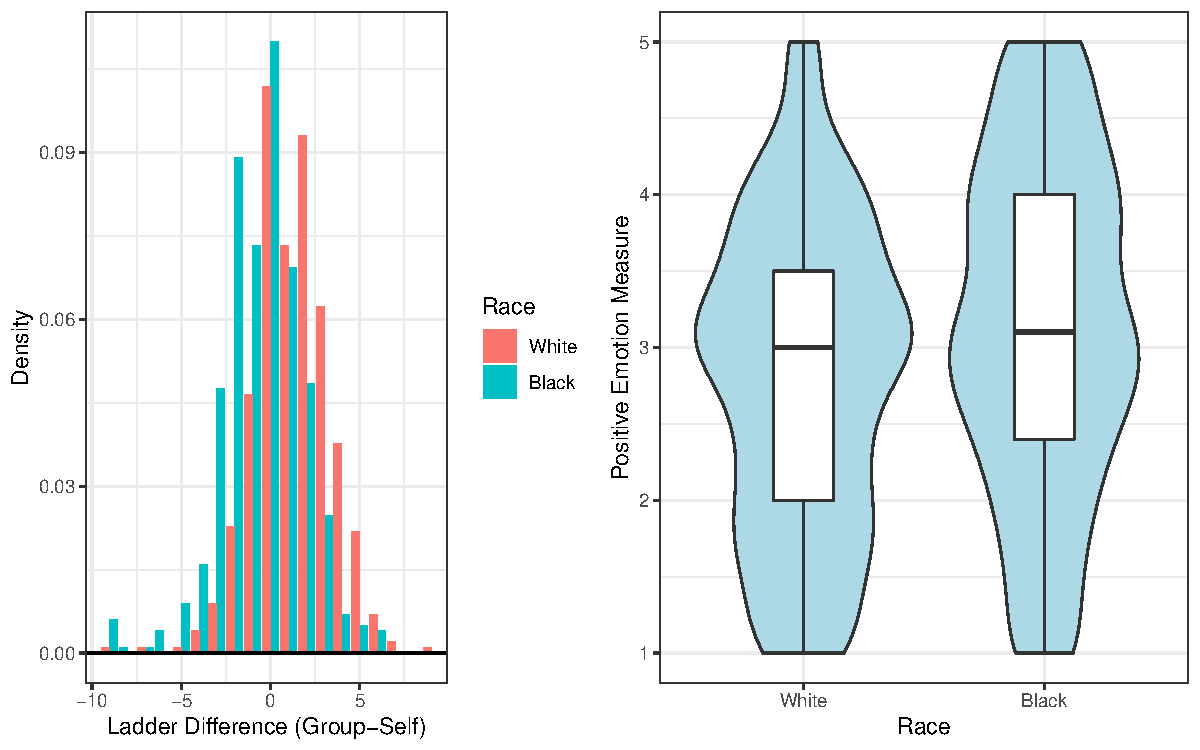
\includegraphics{finalExam-025}
\caption{Plots summarizing ladder difference and the positive emotion measures
by race.} \label{Fig:marginal1}
\end{figure}

In Figure \ref{Fig:boxplot1}, we see there is some
association in Ladder Difference score and Positive 
Emotions. While Black participants have consistent median
Positive Emotions, White participants appear to have higher
Positive Emotion scores when they rate themselves higher 
than the group (LadderDif$<$0) and lower Positive Emotion
scores when they rate themselves lower than the group
(LadderDif$>$0). 
\begin{Schunk}
\begin{Sinput}
> dat.wb$LadderDif.factor<-factor(dat.wb$LadderDif)
> ggplot(data=dat.wb,aes(x=LadderDif.factor,y=PosEmo,fill=Race))+
+ geom_boxplot(position = position_dodge(preserve = "single"))+
+ theme_bw()+
+ xlab("Ladder Difference (Group-Self)")+
+ ylab("Positive Emotion Measure")
\end{Sinput}
\end{Schunk}
\begin{figure}[H]
\centering
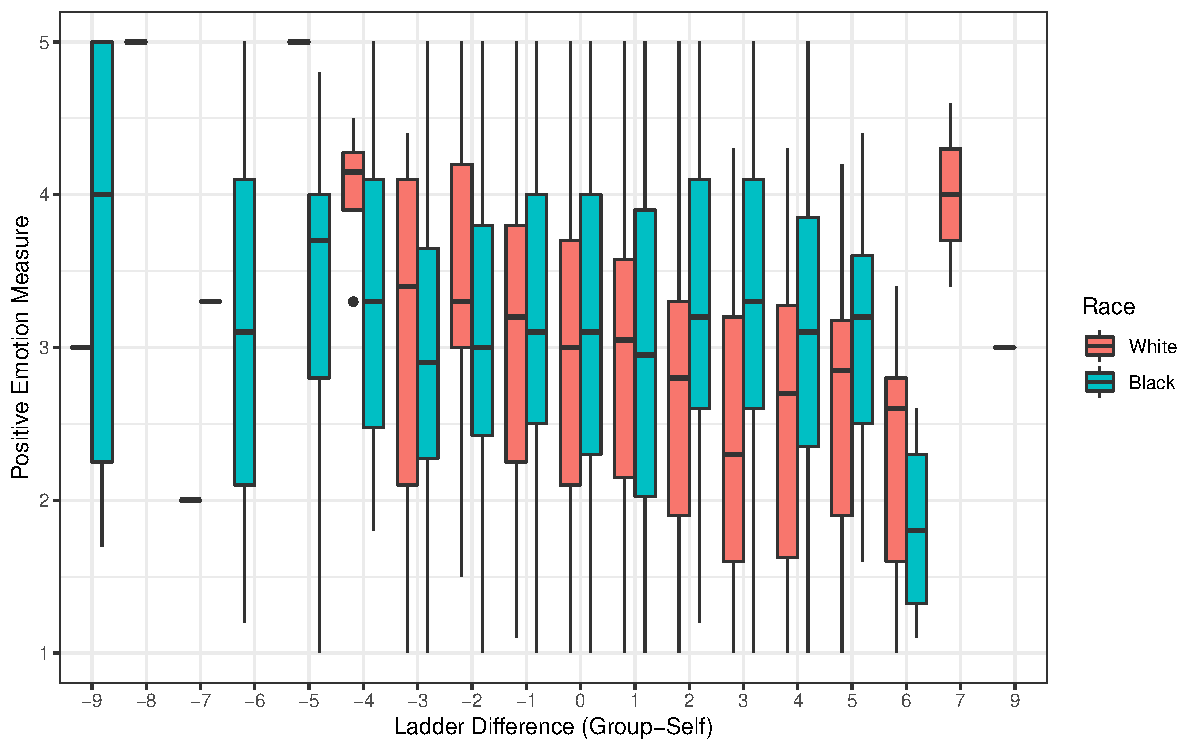
\includegraphics{finalExam-027}
\caption{Plots summarizing ladder difference and the positive emotion measures
by race.} \label{Fig:boxplot1}
\end{figure}
\end{enumerate}
Overall, this review excelled in its ability to discuss its figures and create a story for the data. However, it could be improved in the way it presents the data in figures. For example when looking at figure 3, the two graphs together are not presenting the same data or using the same axes, therefore it is confusing to present them side-by-side. It could be more complementary to present the combined histogram for white and black identifying individuals and then use two separated histograms (one histogram for each race) side-by-side. The violin plot, because it is still very informative, could be presented below. Also, it may be useful to present the analyses of the figures after the figures instead of before, but still on the same page. While this is a knit-picky formatting issue, it makes the data a lot easier to read and the information easier to follow. It generates a good flow for the overall project. When analyzing the figures, it is also important to be careful with the claims that are being made. While it is important to draw information from the figures, claims such as the one on line 253 should be backed up with more evidence or followed up on. Also, the coding in some places could've been more concise, for example on line 217 there wasn't necessarily a need to introduce dat.matched. Also, the discussion of the NA variables was impressive and a good critique of the data, however it could be helpful to explore this further or create a copy of the data frame with the NA variables removed, allowing other researchers to perform their own analyses if needed. 
\item Is there evidence that the ladder difference score differs for Black and White participants?
\newline To determine whether or not there is a statistically significant difference in ladder difference scores for Black and White participants, I'll conduct a Two-Sample T Test. 
\textbf{Hypotheses:}
The null hypothesis is that the mean ladder difference scores for black and white participants are equal. The alternative hypothesis is the the mean ladder difference scores for black and white participants are not equal. 
\newline \textbf{Assumptions:} The assumptions for a Two-Sample T-test is that the two random samples are independent, the two population distributions are Gaussian, and the two population distributions have to have the same variance. 
\begin{enumerate}
\item \textbf{Independent Random Samples:} The data was collected from an online AmazonTurk survey. While we can't prove that these observations are all independent, for the purposes of our research we will assume that each observation is a different person. 
\item \textbf{Gaussian Population Distributions:} 
\begin{figure}[H]
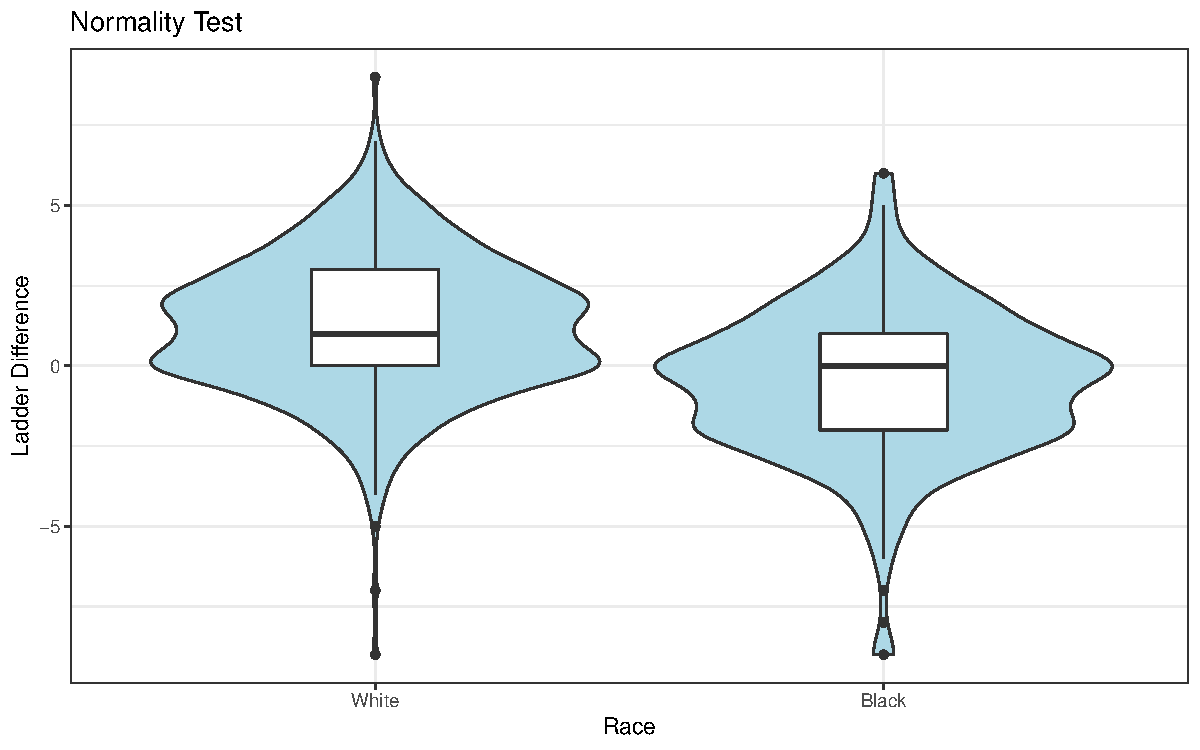
\includegraphics{finalExam-028}
\end{figure}
While the two samples are bimodal, they are still relatively normal. Therefore, we can proceed with our analyses using a two-sample test. 
\item \textbf{Equal Population Variances:}
\begin{Schunk}
\begin{Sinput}
> bartlett.test(dat.wb$LadderDif, dat.wb$Race)
\end{Sinput}
\begin{Soutput}
	Bartlett test of homogeneity of variances

data:  dat.wb$LadderDif and dat.wb$Race
Bartlett's K-squared = 3.1955, df = 1, p-value = 0.07384
\end{Soutput}
\end{Schunk}
Our p-value is 0.074, which is greater than 0.05 and therefore not statistically significant. Therefore, we fail to reject the null which implies that there are equal population variances. 
Below, we can run the two-sample t-test to determine if there is evidence that the ladder difference score differs for black and white participants.
\end{enumerate}

\begin{Schunk}
\begin{Sinput}
> t.test(dat.wb$LadderDif, as.numeric(dat.wb$Race), alternative = "two.sided")
\end{Sinput}
\begin{Soutput}
	Welch Two Sample t-test

data:  dat.wb$LadderDif and as.numeric(dat.wb$Race)
t = -15.161, df = 1095.2, p-value < 2.2e-16
alternative hypothesis: true difference in means is not equal to 0
95 percent confidence interval:
 -1.329581 -1.024874
sample estimates:
mean of x mean of y 
0.3376238 1.5148515 
\end{Soutput}
\end{Schunk}
Our p-value is essentially zero, which is less than 0.05. This means that we can reject our null hypothesis and that the true difference in means is not equal to 0. This implies that there is evidence that the ladder difference score differs for black and white participants. Especially in the sense that white participants may feel more positive emotion than black participants. The 95\% confidence interval given, (-1.329581, -1.024874), also does not contain 0, which further strengthens our results. 

\item Is there evidence that Black and White participants report different levels of positive emotions?
\newline To determine whether or not there is a different level of positive emotions for Black and White participants, we can run a two-sample t-test. 
\newline \textbf{Hypotheses:}The null hypothesis is that average level of positive emotions for black participants and white participants are equal. The alternative hypothesis is that the average level of positive emotions for black and white participants are not equal. 
\newline \textbf{Assumptions:} The assumptions for a Two-Sample T-test is that the two random samples are independent, the two population distributions are Gaussian, and the two population distributions have to have the same variance. 
\begin{enumerate}
\item \textbf{Independent Random Samples:} The data was collected from an online AmazonTurk survey. While we can't prove that these observations are all independent, for the purposes of our research we will assume that each observation is a different person. 
\item \textbf{Gaussian Population Distributions:} 
\begin{figure}[H]
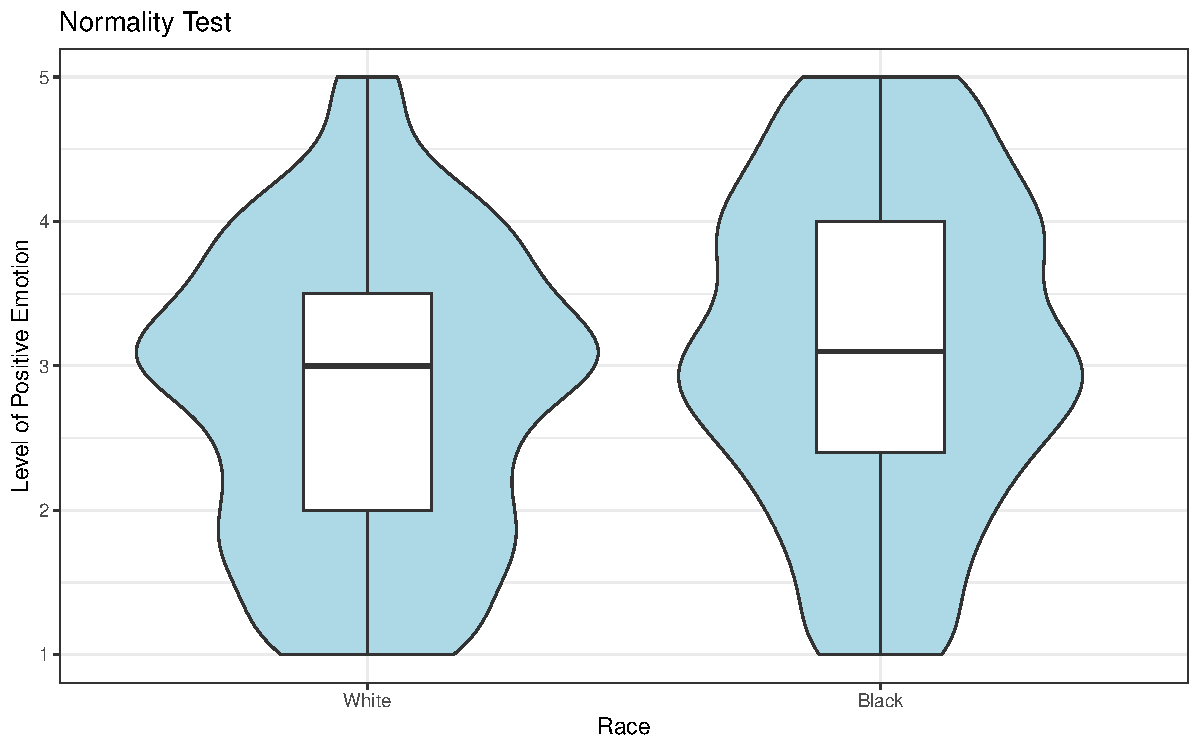
\includegraphics{finalExam-031}
\end{figure}
The two samples are relatively normal, even though they are slightly bimodel. Therefore, we can proceed with our analyses using a two-sample test. 
\item \textbf{Equal Population Variances:}
\begin{Schunk}
\begin{Sinput}
> bartlett.test(dat.wb$PosEmo, dat.wb$Race)
\end{Sinput}
\begin{Soutput}
	Bartlett test of homogeneity of variances

data:  dat.wb$PosEmo and dat.wb$Race
Bartlett's K-squared = 2.4697, df = 1, p-value = 0.1161
\end{Soutput}
\end{Schunk}
Our p-value is 0.1161, which is greater than 0.05 and therefore not statistically significant. Therefore, we fail to reject the null which implies that there are equal population variances.
\end{enumerate}
Below, we can run the two-sample t-test to determine if there is evidence that the ladder difference score differs for black and white participants.
\begin{Schunk}
\begin{Sinput}
> t.test(dat.wb$PosEmo, as.numeric(dat.wb$Race), alternative = "two.sided")
\end{Sinput}
\begin{Soutput}
	Welch Two Sample t-test

data:  dat.wb$PosEmo and as.numeric(dat.wb$Race)
t = 39.148, df = 1431.4, p-value < 2.2e-16
alternative hypothesis: true difference in means is not equal to 0
95 percent confidence interval:
 1.377405 1.522723
sample estimates:
mean of x mean of y 
 2.964916  1.514851 
\end{Soutput}
\end{Schunk}
Our p-value is essentially zero, which is less than 0.05. This means that we can reject our null hypothesis and that the true difference in means is not equal to 0. This implies that there is evidence that black and white participants report different levels of positive emotion. This is important to investigate further, and see if this effect combined with the effect of the previous test for ladder difference could be related. The 95\% confidence interval given, (1.377405, 1.522723), also does not contain 0, which further strengthens our results. 

\item Fit a linear regression model that predicts a participant's positive emotions by their ladder difference, race, and their interaction while controlling for income, education, age, and gender. Interpret the coefficients in the context of the research. Ensure to check the assumptions of the model and fix any issues.

\begin{Schunk}
\begin{Sinput}
> mod<-lm(PosEmo~LadderDif+Race+LadderDif*Race+as.numeric(Income)+as.numeric(Edu)+as.numeric(Age)+as.factor(Gender), data=dat.wb)
> mod1<-lm(PosEmo~LadderDif+Race+LadderDif*Race+Income+Edu+Age+Gender, data=dat.wb)
> summary(mod)
\end{Sinput}
\begin{Soutput}
Call:
lm(formula = PosEmo ~ LadderDif + Race + LadderDif * Race + as.numeric(Income) + 
    as.numeric(Edu) + as.numeric(Age) + as.factor(Gender), data = dat.wb)

Residuals:
    Min      1Q  Median      3Q     Max 
-2.4214 -0.7579  0.0278  0.8014  2.3960 

Coefficients:
                     Estimate Std. Error t value Pr(>|t|)    
(Intercept)          2.737812   0.155608  17.594  < 2e-16 ***
LadderDif           -0.087340   0.022585  -3.867 0.000117 ***
RaceBlack            0.272822   0.078469   3.477 0.000529 ***
as.numeric(Income)   0.069436   0.020928   3.318 0.000940 ***
as.numeric(Edu)     -0.052003   0.025687  -2.025 0.043182 *  
as.numeric(Age)      0.004569   0.002110   2.166 0.030561 *  
as.factor(Gender)2  -0.139186   0.065372  -2.129 0.033488 *  
as.factor(Gender)3  -1.145465   1.038909  -1.103 0.270482    
as.factor(Gender)4   0.663265   1.035783   0.640 0.522091    
LadderDif:RaceBlack  0.072032   0.029451   2.446 0.014623 *  
---
Signif. codes:  0 ‘***’ 0.001 ‘**’ 0.01 ‘*’ 0.05 ‘.’ 0.1 ‘ ’ 1

Residual standard error: 1.034 on 999 degrees of freedom
  (1 observation deleted due to missingness)
Multiple R-squared:  0.06635,	Adjusted R-squared:  0.05794 
F-statistic: 7.888 on 9 and 999 DF,  p-value: 2.588e-11
\end{Soutput}
\end{Schunk}

We can check our assumptions of a linear model to see if our regression is valid before we can draw conclusions. 

\textbf{Assumptions:}
\begin{enumerate}
\item \textbf{Valid Model} This is a valid model because it maps our variables of interest onto our outcome variable and controls for identifying variables. 

\item \textbf{Linearity of Relationship}
\begin{figure}[H]
\begin{Schunk}
\begin{Sinput}
> ggdat<-data.frame(y=dat.wb$PosEmo,
+                   x=dat.wb$LadderDif,
+                   treatment=dat.wb$Race)
> ggplot(data=ggdat,aes(x=x,y=y))+
+   geom_point(aes(color=treatment))+
+   geom_smooth(method = "loess")+
+   xlab("Ladder Difference")+
+   ylab("Positive Emotion")+
+   ggtitle("Linearity Test")+
+   labs(color="")+
+   theme_bw()
\end{Sinput}
\end{Schunk}
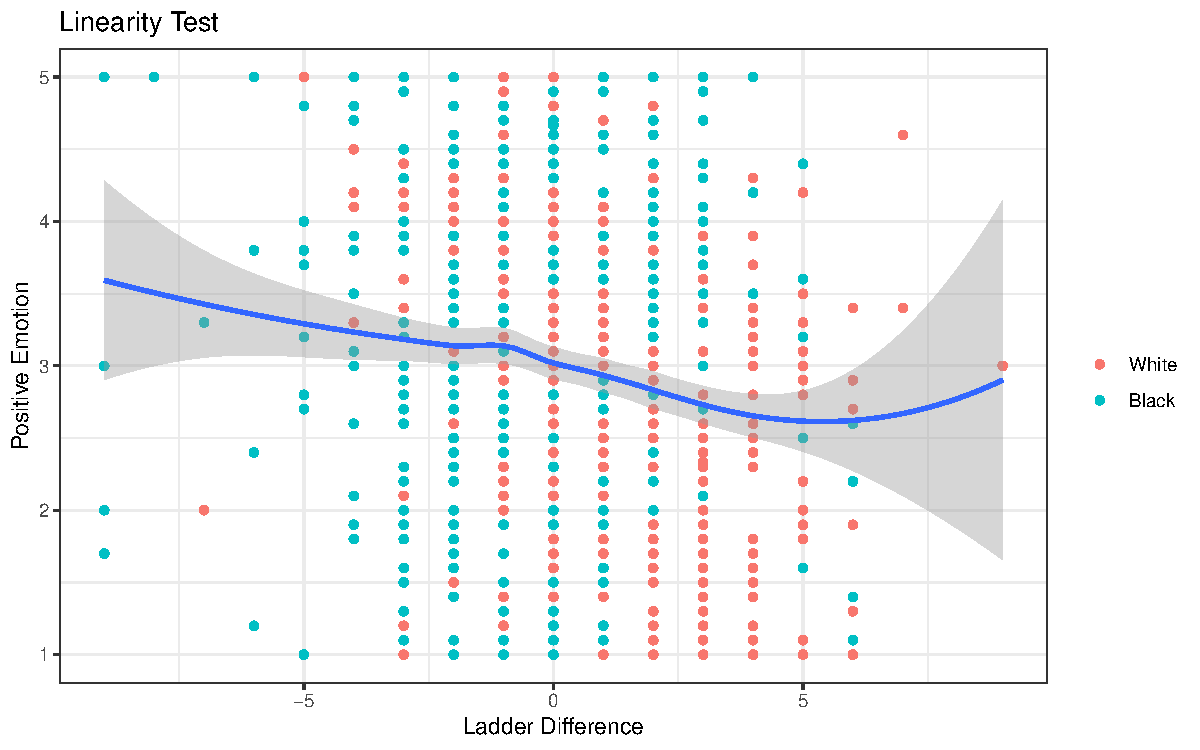
\includegraphics{finalExam-035}
\end{figure}
We see that the data follows a general linear trend with only one minor bump in the regression line. 

\item \textbf{Errors are Independent}
\item \textbf{Errors are Normally Distributed}
\item \textbf{Errors have Constant Variance}
\item \textbf{No Outliers}

\begin{Schunk}
\begin{Sinput}
> par(mfrow=c(2,2))
> plot(mod)
\end{Sinput}
\end{Schunk}
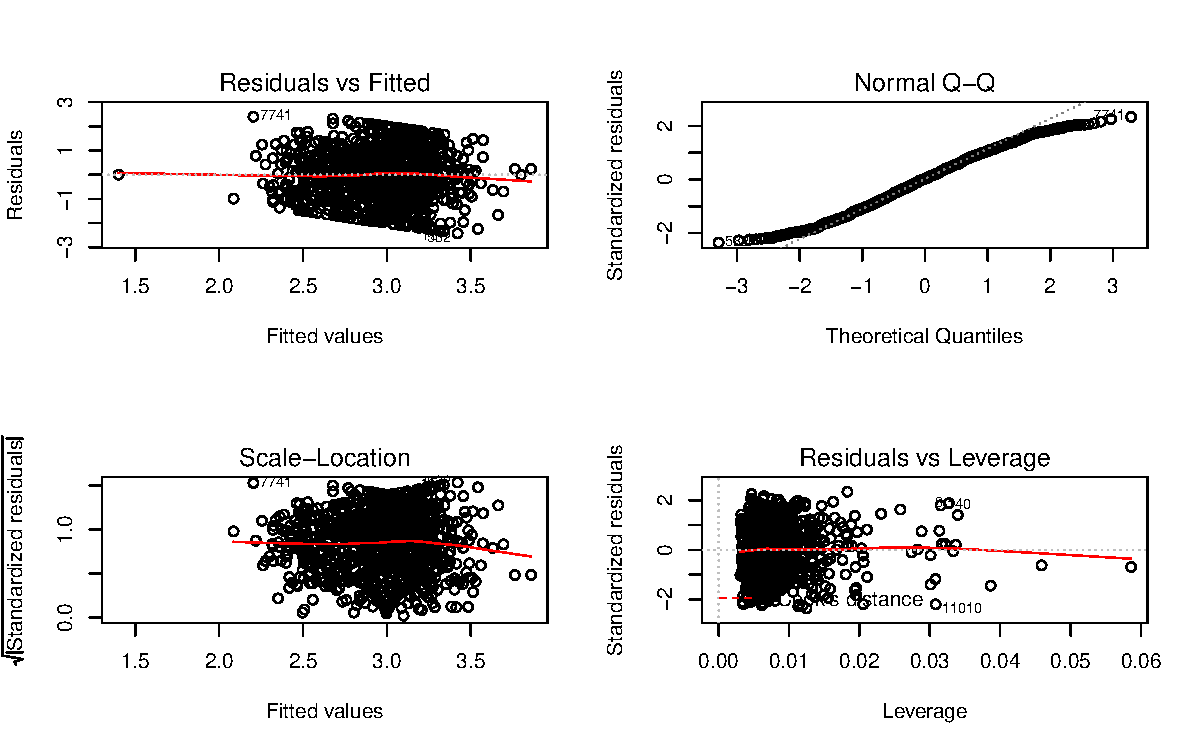
\includegraphics{finalExam-036}
\newline We see that there is no pattern in the residual plot, there are few outliers, there is no severe normality departures, few outliers, and no leverage points. 

\item \textbf{7. No missing predictors}
We know that large R squared indicates that we've captured more of the variability. 
Our R-squared value is 0.05794. Because the value is low, we can assume that we most likely need to add more predictors to our model. However, this doesn't completely negate the validity of the other predictors and controls we have already included. 
\item \textbf{8. No multicollinearity}
\begin{Schunk}
\begin{Sinput}
> library(car)
> vif(mod)
\end{Sinput}
\begin{Soutput}
                       GVIF Df GVIF^(1/(2*Df))
LadderDif          2.811702  1        1.676813
Race               1.452015  1        1.204996
as.numeric(Income) 1.272712  1        1.128145
as.numeric(Edu)    1.193981  1        1.092694
as.numeric(Age)    1.250200  1        1.118123
as.factor(Gender)  1.015804  3        1.002617
LadderDif:Race     2.340658  1        1.529921
\end{Soutput}
\end{Schunk}
None of these predictors have a VIF value greater than 5 which indicates that none of these predictors are too correlated with the other.
\end{enumerate}
Now that we have checked our assumptions for the tests, we can assess and interpret the coefficients of our model. 

We see from our model that LadderDif, Race (a dummy variable), and income are highly statistically significant with positive emotion level, as well as the intercept. We can interpret these coefficients to determine the effect of each predictor/control on positive emotion level. 

\textbf{Coefficients}
\begin{enumerate}
\item \textbf{LadderDif Coefficient: -0.087340} LadderDif tells us that as ladder difference increases by 1, positive emotion levels decrease by 0.087, a small, but significant decrease. 
\item \textbf{RaceBlack: 0.272822} RaceBlack is a dummy variable where the variable is 0 when the person identifies as White and 1 when the person identifies as Black. Therefore, we can interpret the coefficient as saying that people who as being Black see an increase in positive emotion of .2728. 
\item \textbf{Income: 0.069436} Income as a numeric value tells us that as a person's income level increases by 1, their positive emotion level increases by 0.0694. 
\item \textbf{Interaction Term - LadderDif*RaceBlack: 0.072032} The interaction term between ladder difference and race is also statistically significant at the 5\% level, but not highly statistically significant. This tells us that identifying as not being Black and increasing your ladder difference by 1 level increases your positive emotion level by 0.0720 more than if someone identified as being Black. Race is therefore an important factor in determining the magnitude of the effect of an individual's ladder difference level on their positive emotion level. 
\end{enumerate}

\item Provide the marginal effects of ladder difference at specified race; e.g., Black and White.  Ensure to provide a plot of the marginal means by race to provide a visual of the marginal effects. Interpret this output in the context of the research.

\begin{Schunk}
\begin{Sinput}
> #install.packages("ggeffects")
> library(ggeffects)
> marginal.SES<-ggeffect(mod1,c("LadderDif","Race"))
> plot(marginal.SES)
> library(margins)
> margins(mod1, variables = "LadderDif",
+         at=list(Race=c("Black", "White")))
\end{Sinput}
\begin{Soutput}
 at(Race) LadderDif
    Black  -0.01822
    White  -0.08146
\end{Soutput}
\end{Schunk}
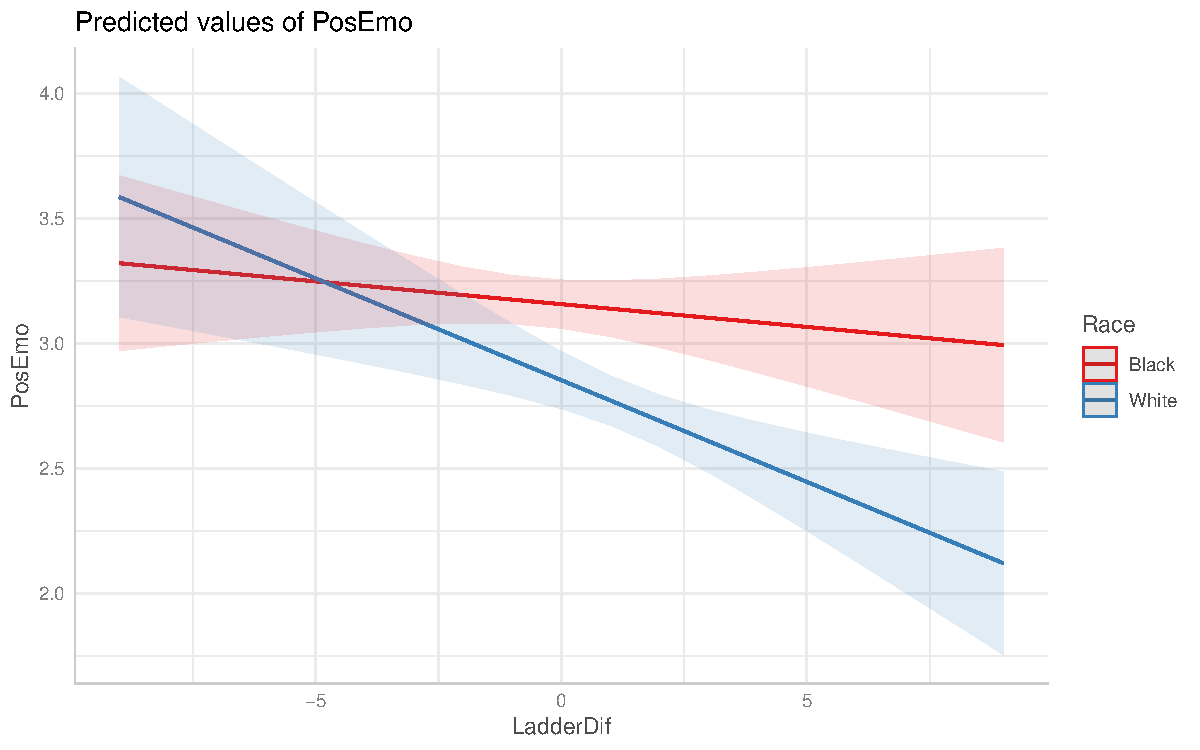
\includegraphics{finalExam-038}
As we can see, using the ggeffects \citep{ggeffects} package, we can plot the predicted values of white and black people based on the ladder difference. As the plot suggests, there is a greater difference between the positive emotion levels of white and black people when ladder differences are farther from zero. This is illustrated by the interaction term in our regression model. 

The magnitude of the marginal effect, given to us using the margins \citep{margins} package is larger for White people than Black people as can be seen in the plot by the steeper slope. The slopes in these cases represent the average marginal effects by race. White people see a greater decrease in positive emotion level as ladder difference increases compared to black people. The difference between the average marginal effects for white people and black people is the value of the interaction term in our original linear regression model. 

\item Report the estimated marginal mean positive emotions by race. Interpret these values.

\begin{Schunk}
\begin{Sinput}
> #install.packages('emmeans')
> library(emmeans)
> mod2<-lm(dat.wb$PosEmo~dat.wb$LadderDif+dat.wb$Race+dat.wb$LadderDif*dat.wb$Race+dat.wb$Income+dat.wb$Edu+dat.wb$Age+dat.wb$Gender)
> emmeans(mod2, c("Race"))
\end{Sinput}
\begin{Soutput}
 Race  emmean    SE  df lower.CL upper.CL
 White   2.99 0.388 917     2.23     3.75
 Black   3.32 0.393 917     2.55     4.09

Results are averaged over the levels of: Income, Edu, Age, Gender 
Confidence level used: 0.95 
\end{Soutput}
\end{Schunk}
\begin{figure}[H]
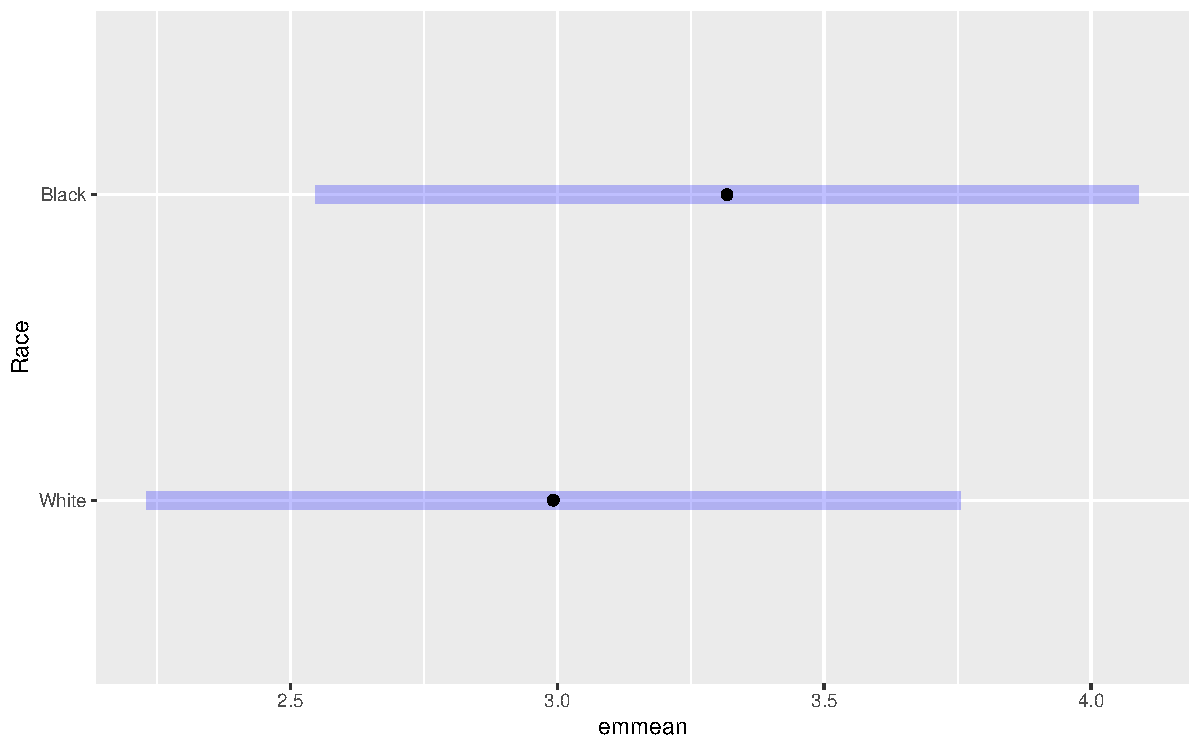
\includegraphics{finalExam-040}
\end{figure}
Using the emmeans package \citep(emmeans), we calculated the estimated marginal mean positive emotions by race and found that the estimated marginal mean for positive emotions for white people was 2.99 and 3.32 for black people. This means that black people tend to have higher positive emotions on average, although since the confidence intervals for white and black people are interacting, these results aren't necessarily significant. As we can see from the plot, there is a large amount of overlap between these groups. 

\item Provide a contrast for the difference of the marginal means of positive emotions across races. Interpret this output in the context of the research.
\begin{Schunk}
\begin{Sinput}
> contrast(emmeans(mod2, c("Race")))
\end{Sinput}
\begin{Soutput}
 contrast     estimate     SE  df t.ratio p.value
 White effect   -0.163 0.0397 917 -4.097  <.0001 
 Black effect    0.163 0.0397 917  4.097  <.0001 

Results are averaged over the levels of: Income, Edu, Age, Gender 
P value adjustment: fdr method for 2 tests 
\end{Soutput}
\end{Schunk}
Our results show us that the white effect is negative and the black effect is positive. In fact, the p-values that are essentially zero for both effects, coupled with the fact that the white and black effect are estimated in equal, opposite directions, tells us that there are significant opposite effects between black and white people when it comes to how race effects their level of positive emotion. 

\item In Homework 1, question 2, we explored how the groups participants self-identified as are strongly 
associated to who they compare themselves when reporting their relative social standing in the United States.
This research was aimed to explain the complex intersections of race and class. In particular, we were curious
about how widespread assumptions that Black=poor and White=wealthy contribute to political polarization, race-related health disparities, and racial resentment -- especially among poor, White people.

This study was in response to a peer-reviewer who suggested that, maybe, people don't necessarily have the same
self-comparison groups. Does the analysis from Homework 1 convince you that this is likely not an issue?
\newline \textbf{Response:}
In Homework 1, question 2, we explored how the groups participants self-identified as are strongly associated to who they compare themselves to when reporting their relative social standing. We found that 96.59\% of white people compared themselves to white people and 80\% of black people compared themselves to black people, while 16.84\% of black people compared themselves to white people and 1.05\% of black people compared themselves to biracial and multiracial people. A Fisher Exact Test shows us that there is strong dependence between self-identified race and comparison group, meaning that people tend to compare themselves to their own race group. These results were similar for groups such as gender, age, and educational attainment level. Therefore, the analysis from homework 1 convinces me that this is likely not an issue. 
\end{enumerate}
%attach bibliography and end document.
\bibliography{bib}
\end{document}
